\documentclass{article}
\usepackage{arxiv}

\usepackage[utf8]{inputenc} % allow utf-8 input
\usepackage[T1]{fontenc}    % use 8-bit T1 fonts
\usepackage{url}            % simple URL typesetting
\usepackage{booktabs}       % professional-quality tables
\usepackage{amsfonts}       % blackboard math symbols
\usepackage{amsmath}
\usepackage{nicefrac}       % compact symbols for 1/2, etc.
\usepackage{microtype}      % microtypography
\usepackage{lipsum}
\usepackage{caption}
\usepackage{graphicx}
\usepackage{minted} 
\usepackage{hyperref}       % hyperlinks
\usepackage{listings}
\usepackage{pgffor}			

\usepackage{xcolor}
\definecolor{bg}{rgb}{0.95, 0.95, 0.92}
\definecolor{deepblue}{rgb}{0,0,0.5}
\definecolor{deepred}{rgb}{0.6,0,0}
\definecolor{deepgreen}{rgb}{0,0.5,0}

\DeclareFixedFont{\ttb}{T1}{txtt}{bx}{n}{10} % for bold
\DeclareFixedFont{\ttm}{T1}{txtt}{m}{n}{10}  % for normal

\DeclareCaptionFormat{listing}{#1#2#3}
\captionsetup[lstlisting]{format=listing, singlelinecheck=false, margin=0pt, font={sf}}

\lstset{
  numberstyle=\ttm,
  basicstyle=\ttm,
  numbers=left,
  columns=fullflexible,
  frame=top,
  breaklines=true,
  showstringspaces=false,
  postbreak=\mbox{\textcolor{red}{$\hookrightarrow$}\space},
  keywordstyle=\ttb\color{deepblue},
  emph={MyClass,__init__},          
  emphstyle=\ttb\color{deepred},   
  stringstyle=\color{deepgreen},
}


\title{News broadcast analysis}


\author{
	Christine K. C. Cheng
}

\begin{document}
\maketitle

\section{Shot detection}
A score is calculated for each frame using either the sum of absolute differences method or the histogram differences method. Given the mean $\mu$ and standard deviation $\sigma$ of all the scores, a threshold is chosen as $$\text{threshold} = \mu + k\times \sigma$$ where $k$ is an integer. A shot is a series of frames taken by continuously by one camera. A shot change is declared when the value of the score becomes greater than the threshold and then becomes smaller than the threshold (similar to a peak above the threshold line).

\subsection*{Sum of absolute differences}
A score is assigned to each frame by calculating the sum of the absolute differences between consecutive frames for every pixel. This value is then normalized by the size of the frame. When the score of a frame is greater than the threshold, a shot change is declared. This method works quite well with simple videos but it is not robust against movements and changes in lighting.

\subsection*{Histogram differences}
Each frame is converted into a gray-scale image. A histogram with 256 bins, representing all the possible values of a pixel, is created for each frame. Then, a score is assigned by calculating the sum of the absolute differences between histograms of consecutive frames. This method is more robust against small changes in a frame.

\subsection*{Performance}
Let $C$ be the number of correctly identified cuts, $M$ be the number of cuts that are not identified, and $F$ be the number of falsely identified cuts. To evaluate how well the algorithm is detecting the shots, the recall (V), precision (P) and $F_1$ scores for each clip are calculated. They are defined as below.

\begin{equation}
\begin{split}
V &= \frac{C}{C + M} \\
P &= \frac{C}{C + F} \\
F_1 &= \frac{2 \times P \times V}{P + V} \\
\end{split}
\end{equation}

\vspace*{10pt}
\begin{minipage}{0.5\linewidth}
\captionof{figure}{Sum of absolute differences scores of clip 1} \label{fig: clip_1_sad2}
\centering
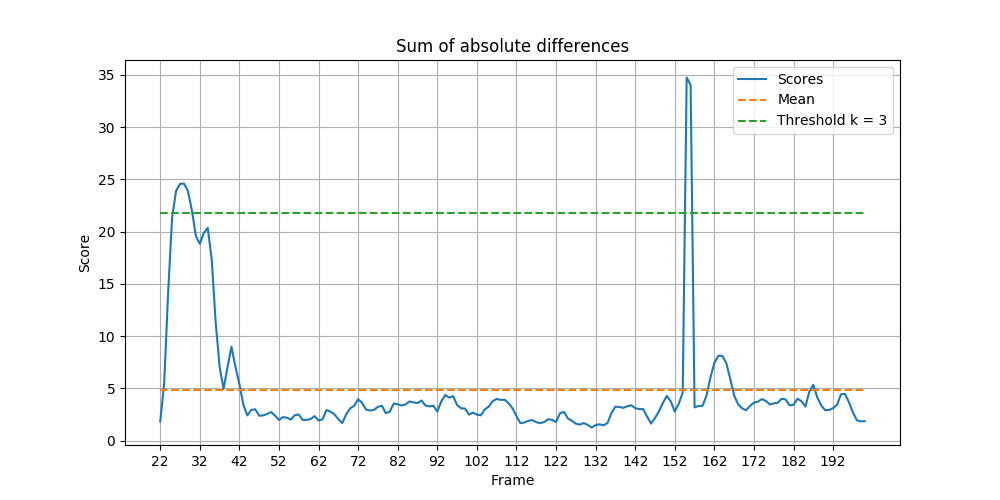
\includegraphics[width=3.5in]{../output/clip_1_score_sad2.png}
\end{minipage}%
\begin{minipage}{0.5\linewidth}
\captionof{figure}{Histogram differences scores of clip 1} \label{fig: clip_1_hd}
\centering
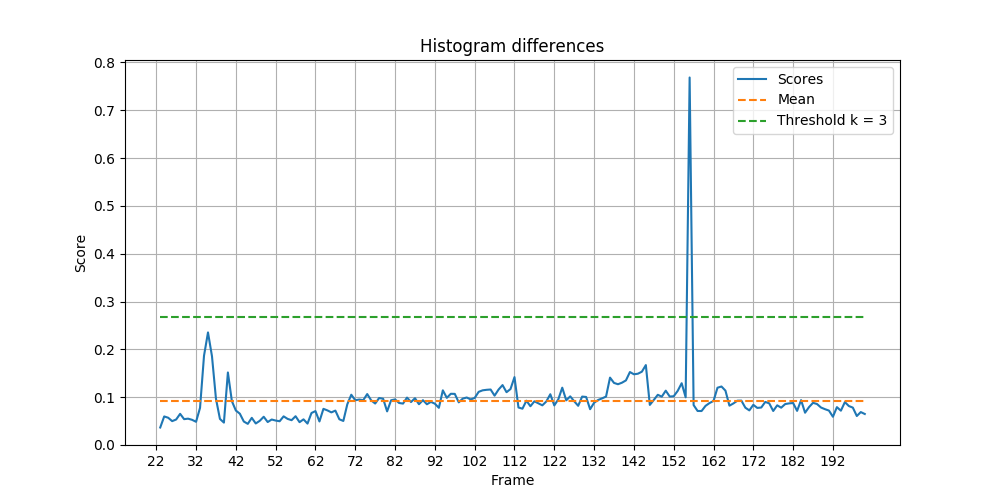
\includegraphics[width=3.5in]{../output/clip_1_score_hd.png}
\end{minipage}

\begin{minipage}{0.5\linewidth}
\captionof{figure}{Sum of absolute differences scores of clip 2} \label{fig: clip_2_sad2}
\centering
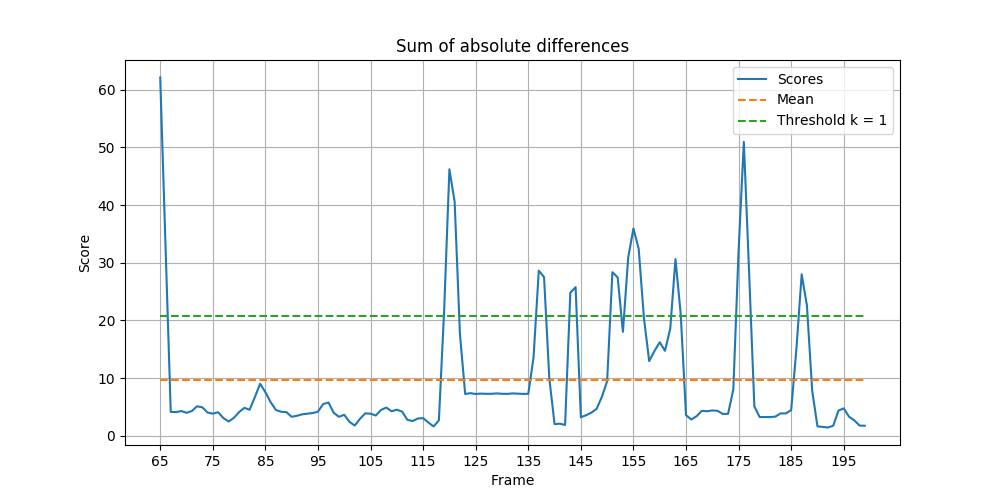
\includegraphics[width=3.5in]{../output/clip_2_score_sad2.png}
\end{minipage}%
\begin{minipage}{0.5\linewidth}
\captionof{figure}{Histogram differences scores of clip 2} \label{fig: clip_2_hd}
\centering
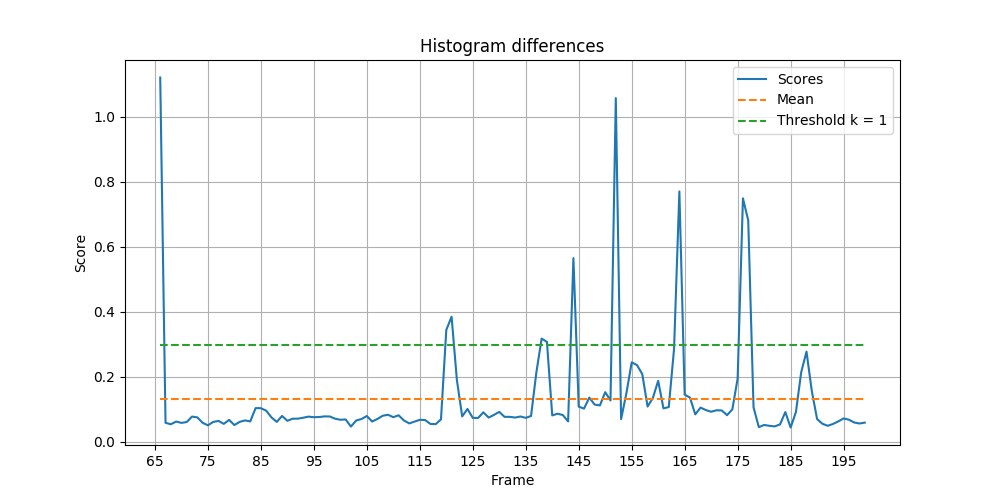
\includegraphics[width=3.5in]{../output/clip_2_score_hd.png}
\end{minipage}

\begin{minipage}{0.5\linewidth}
\captionof{figure}{Sum of absolute differences scores of clip 3} \label{fig: clip_3_sad2}
\centering
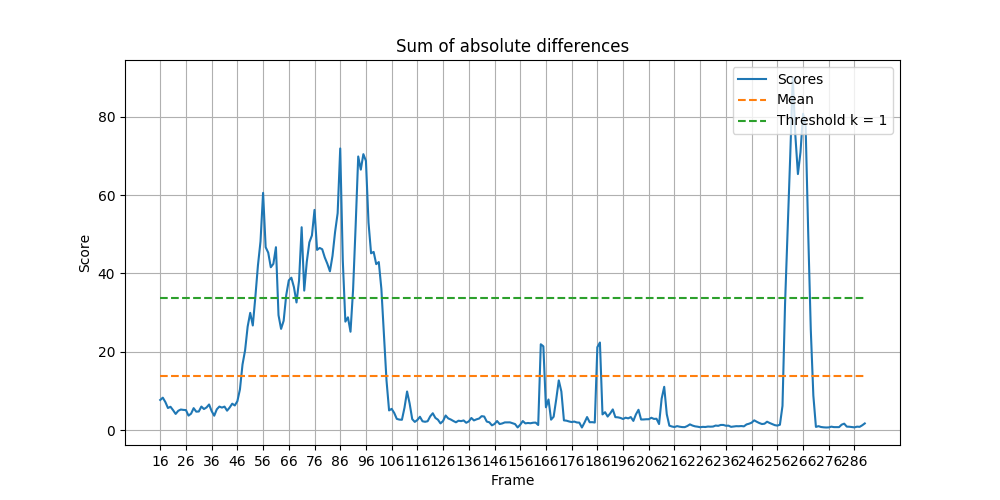
\includegraphics[width=3.6in]{../output/clip_3_score_sad2.png}
\end{minipage}%
\begin{minipage}{0.5\linewidth}
\captionof{figure}{Histogram differences scores of clip 3} \label{fig: clip_3_hd}
\centering
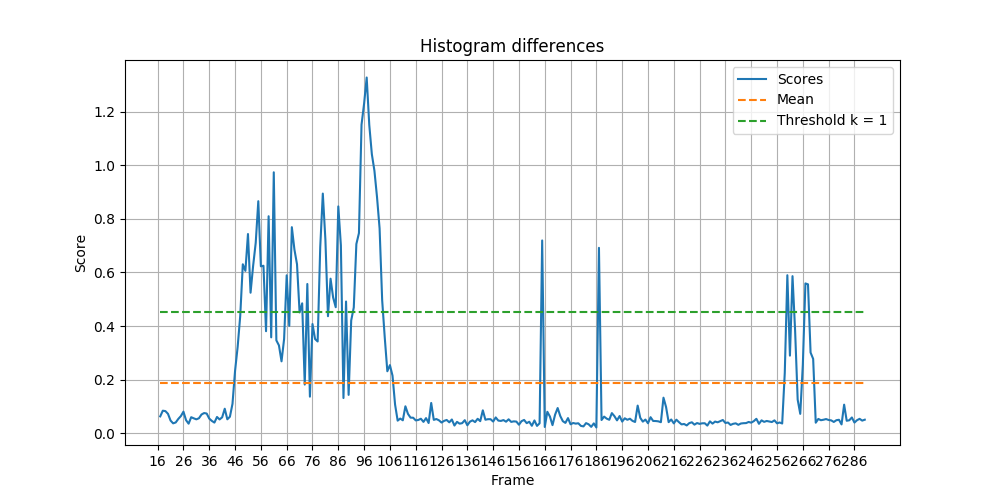
\includegraphics[width=3.6in]{../output/clip_3_score_hd.png}
\end{minipage}
\vspace*{10pt}
 
Table \ref{tab:sad_results} and Table \ref{tab:hd_results} shows the respective scores for both methods. On average, histogram differences achieve a higher score across all three metrics comparing to sum of absolute differences method. For example, the transition from frame 164 (Figure \ref{clip_3_f164}) to frame 165 (Figure \ref{fig: clip_3_f165}) is not detected by the latter but it is by the former. It performs especially better in the montage section in clip 3, where there are frequent shot changes. 

 \begin{table}[h]
 \caption{Shot detection performance with sum of absolute differences}
  \centering
  \begin{tabular}{lllllll}
    \toprule
    Clip		& Correct (C)	& Missed (M)	& Falsely detected (F) 	& Recall (V) 		& Precision (P) 	& $F_1$ \\
    \midrule
    1			& 	1					& 0					& 1 									& 1					& 0.5					& 0.6667 \\
    2			& 	7					& 0					& 2 									& 1					& 0.7778				& 0.8750 \\
    3			& 	5					& 16					& 0 									& 0.2381			& 1						& 0.3846	\\
    \bottomrule
  \end{tabular}
  \label{tab:sad_results}
\end{table}

\begin{table}[h]
 \caption{Shot detection performance with histogram differences}
  \centering
  \begin{tabular}{lllllll}
    \toprule
    Clip		& Correct (C)	& Missed (M)	& Falsely detected (F) 	& Recall (V) 		& Precision (P) 	& $F_1$ \\
    \midrule
    1			& 	1					& 0					& 0 									& 1					& 1						& 1	\\
    2			& 	6					& 1					& 1 									& 0.8571			& 0.8571				& 0.8571	\\
    3			& 	15				& 6					& 1 									& 0.7142			& 0.9375				& 0.8118	\\
    \bottomrule
  \end{tabular}
  \label{tab:hd_results}
\end{table}

\begin{minipage}{0.5\linewidth}
\captionof{figure}{Frame 164 of clip 3} \label{clip_3_f164}
\centering
\includegraphics[width=3in]{../original_data/clip_3/0164.jpg}
\end{minipage}%
\begin{minipage}{0.5\linewidth}
\captionof{figure}{Frame 165 of clip 3} \label{fig: clip_3_f165}
\centering
\includegraphics[width=3in]{../original_data/clip_3/0165.jpg}
\end{minipage}
\vspace*{10pt}

The relevant code is in \texttt{shot.py}. To get the graphs of shot detection, run the command below. 
\begin{minted}[bgcolor=bg]{sh}
python3 run.py shot_detection -t <type> -i <path to frames>
\end{minted}

To add shot numbers into frames, run the command below. The shot number will appear on the bottom left corner of each frame.
\begin{minted}[bgcolor=bg]{sh}
python3 run.py add_shot_numbe -i <input directory> -o <output directory> 
-k <k for thresholding>
\end{minted}

\section{Logo detection}
Template matching is an object detection algorithm which is translation invariant but not scale or rotation invariant. As we are detecting the news company's logo, we can assume that the target of detection will be in a known orientation. Due to the possibility that there may be multiple occurrences of the logo in a frame, we cannot simply match SIFT features between the logo template and a frame. Template matching is run on templates of different sizes because the size of the logo in a frame is unknown. Then, a score is calculated for all the matches by normalized cross-correlation. The normalized version is chosen because brighter patches will not have a higher score. Also, the score obtained will be in the range [0, 1] and this makes choosing a threshold more intuitive. As the logo of the template and the one in the frame might be slightly different, possibly due to the differences in resolutions or styles, a looser threshold is first used to filter out the irrelevant matches. 

For each match, if its score is greater than the loose threshold, it is kept. Then, the algorithm checks if that particular match is a slight translation of a match we have a already decided to keep. If it is, the match is discarded. This prevents having multiple boxes around one logo. Afterwards, SIFT descriptors are calculated for the remaining matches and a score is calculated using feature matching and Lowe's ratio test with the logo template. If a match's score is above a tighter threshold, it is declared as a match of the template and a box is put around the match.

The logo detection was the most difficult part of the project for me. I originally only did one pass with either normalized cross-correlation or SIFT feature matching. However, this led to fairly poor results, with the algorithm often unable to detect multiple logos and including many irrelevant matches. Therefore, the two passes approach, first with a looser threshold using normalized cross-correlation and then a tighter threshold with SIFT feature matching, is used. As can be seen in Figure \ref{fig: logo_good}, the algorithm can detect multiple logos. In hindsight, it would have been more efficient to scale down the images to multiple scales instead of scaling down the templates. This is because sliding the template across the image takes much longer than resizing every frame to different scales.

\vspace*{20pt}
\begin{minipage}{0.5\linewidth}
\captionof{figure}{Logo detection on frame 104 of clip 1} \label{fig: logo_bad}
\centering
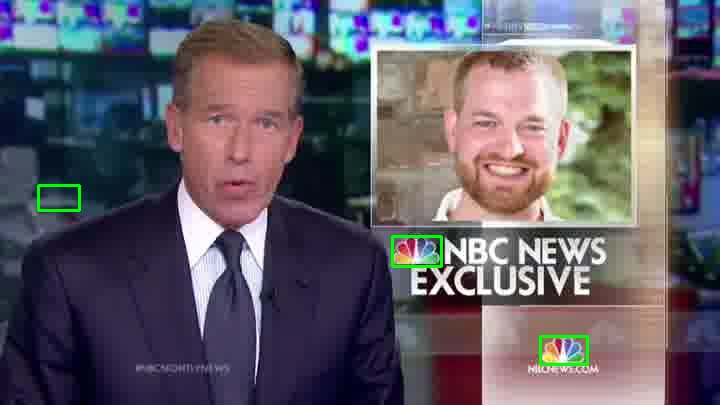
\includegraphics[width=2.5in]{../output/clip_1_logo/104.jpg}
\end{minipage}
\begin{minipage}{0.5\linewidth}
\captionof{figure}{Logo detection on frame 52 of clip 1} \label{fig: logo_good}
\centering
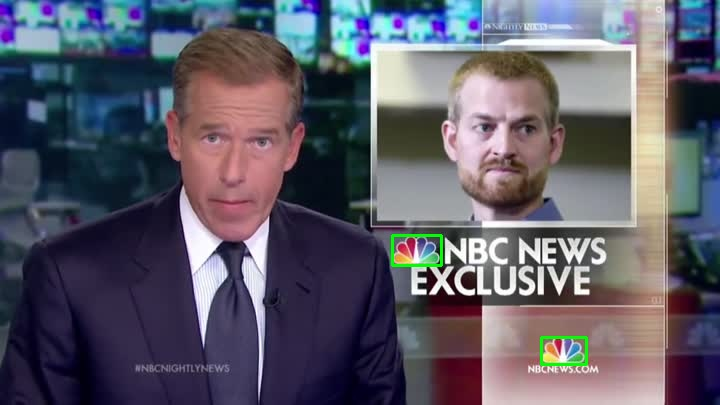
\includegraphics[width=2.5in]{../output/clip_1_logo/052.jpg}
\end{minipage}
\vspace*{10pt}

The relevant code is in \texttt{logo.py}. To run logo detection, run the command below.
\begin{minted}[bgcolor=bg]{sh}
python3 run.py logo_detection -i <input directory> -o <output directory>
-d <logo path> -t <min threshold for NCC>
\end{minted}

\section{Face detection and tracking}
There are 260 images in the female and male classes respectively. Each image is accompanied by a \texttt{.mat} file specifying the coordinates of the left eye, right eye, nose and mouth. The following rules are used to crop the images in order to obtain the faces.
\begin{equation}
\begin{split}
start_x &= left~eye_x - 0.5\times(right~eye_x - left~eye_x) \\
end_x &= right~eye_x + 0.5\times(right~eye_x - left~eye_x) \\
start_y &= eyes_y - (mouth_y - eyes_y) \\
end_y &= mouth_y + (mouth_y - eyes_y) \\
\end{split}
\end{equation}
The relevant code for face cropping is in \texttt{crop\_images()} in \texttt{face.py}.

The initial attempt to detect faces is to use skin detection - trying to filter out skin in images. Figure \ref{fig: rgb} and Figure \ref{fig: hsv} show the color distributions of faces in RGB and HSV color spaces. The HSV color space has narrower distributions, especially with hue. Although this method works sometimes as seen in Figure \ref{fig: hsv_good}, it is not successful in general. It fails to detect a large area of the face of the man on the right in Figure \ref{fig: hsv_bad} and includs a lot of the background.This model is especially poor when other things in the frame are very similar to human skin tone.

\vspace*{20pt}
\begin{minipage}{0.5\linewidth}
\captionof{figure}{RGB distribution of fe male training images} \label{fig: rgb}
\centering
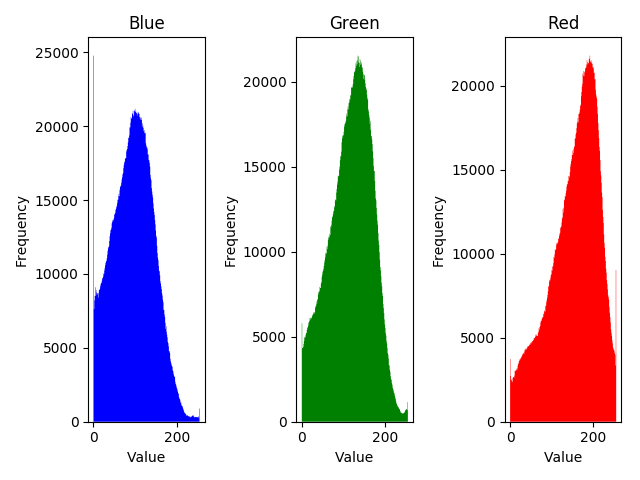
\includegraphics[width=2.5in]{../output/f_train_rgb_distributions.png}
\end{minipage}%
\begin{minipage}{0.5\linewidth}
\captionof{figure}{HSV distribution of female training images} \label{fig: hsv}
\centering
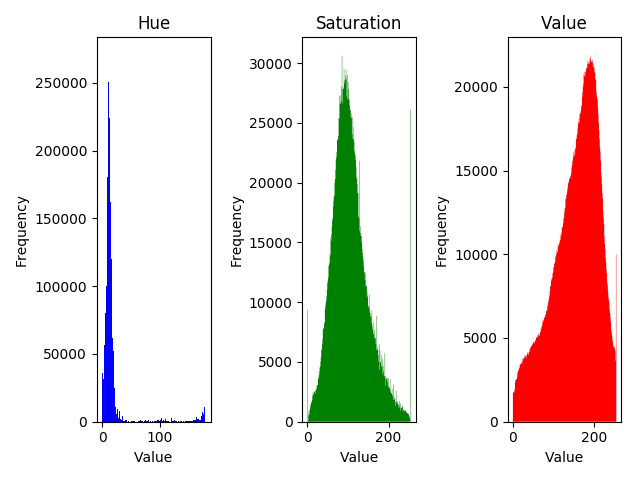
\includegraphics[width=2.5in]{../output/f_train_hsv_distributions.png}
\end{minipage}

\begin{minipage}{0.5\linewidth}
\captionof{figure}{HSV colour detection on frame 160 of clip 1} \label{fig: hsv_good}
\centering
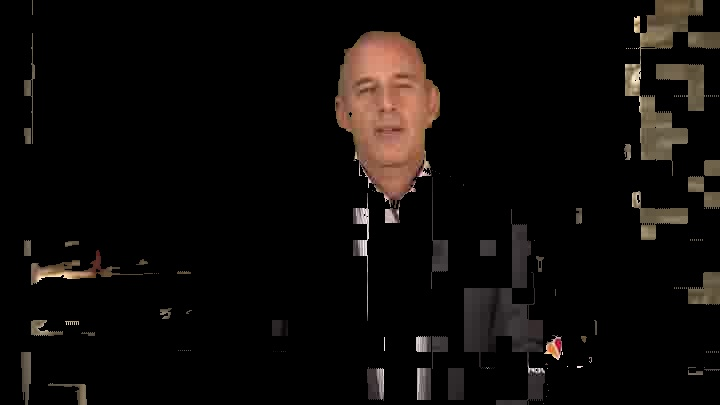
\includegraphics[width=2.5in]{../output/clip_1_hsv/160.jpg}
\end{minipage}
\begin{minipage}{0.5\linewidth}
\captionof{figure}{HSV colour detection on frame 50 of clip 1} \label{fig: hsv_bad}
\centering
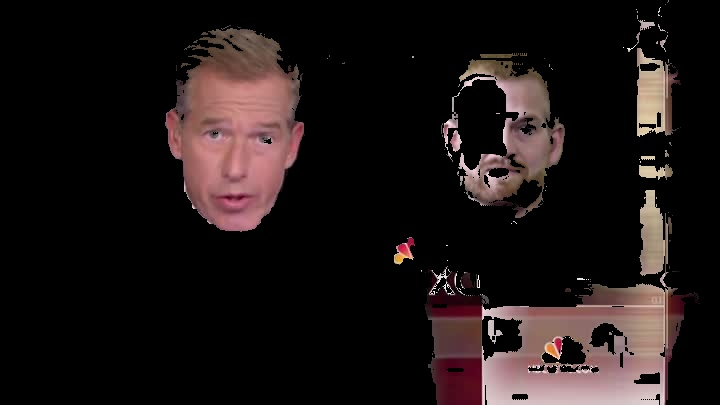
\includegraphics[width=2.5in]{../output/clip_1_hsv/050.jpg}
\end{minipage}
\vspace*{10pt}

The relevant code for HSV face detection is in \texttt{visualize\_distributions()} and \texttt{face\_detection\_hsv()} in \texttt{face.py}.

I ended up using \texttt{cv2.CascadeClassifier} for detecting faces. The full name of this classifier is Haar feature-based cascade classifier for object detection. It is a OpenCV pre-trained classifier for face stored in an XML file. It works fairly well. It has no trouble detecting multiple people in a frame or people of colour, like in Figure \ref{fig: face_good}. However, it is sometimes unable to detect faces in a certain position. The detector was unable to detect the person on the left in any of the frames he appeared in that particular position in Figure \ref{fig: face_bad}.

After obtaining the faces in a frame, for each face in the current frame, the SIFT descriptors are found. Then, they are matched to the SIFT descriptors of each faces in the previous frame using feature matching and Lowe's ratio test. Then, a score is obtained from the number of matches. If the score is above a set threshold, the algorithm declares that the face we are looking at is found in the previous frame and we will display the index assigned to that particular face in the previous frame. If the face is not found, we assign a new index to the face.

\vspace*{10pt}
\begin{minipage}{0.5\linewidth}
\captionof{figure}{Face detection on frame 69 of clip 2} \label{fig: face_good}
\centering
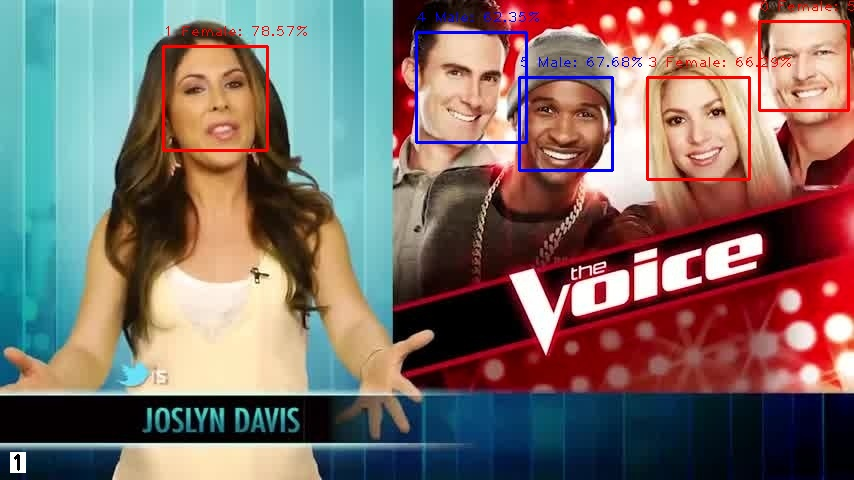
\includegraphics[width=2.5in]{../output/clip_2/069.jpg}
\end{minipage}
\begin{minipage}{0.5\linewidth}
\captionof{figure}{Face detection on frame 110 of clip 1} \label{fig: face_bad}
\centering
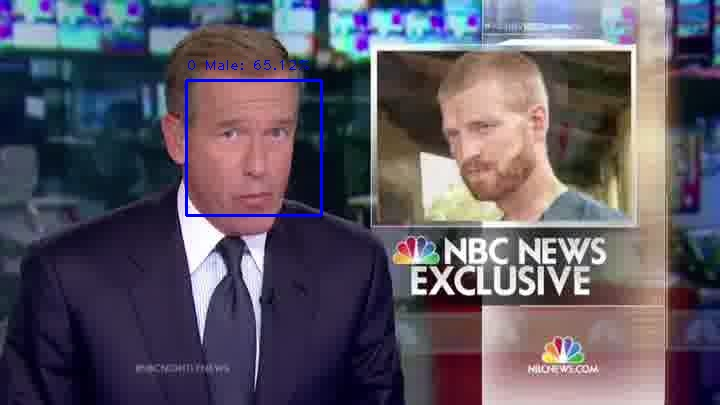
\includegraphics[width=2.5in]{../output/clip_1_face/110.jpg}
\end{minipage}
\vspace*{10pt}

\section{Gender classification}
90\% of the images (234 images from each class) are used for training, whereas the other 10\% (26 images from each class) are used for testing the accuracy of the model.

\subsection*{SVM}
The SIFT descriptors of the training images are passed into the SVM model for training.
For each detected face, the SIFT descriptors are extracted and fed to the trained SVM model. Then, a prediction for each descriptor is obtained. If more descriptors are predicted as female than male, the image is classified as female. If more descriptors are predicted as male than female, the image is classified as male. If there are equal number of descriptors being predicted as both female and male, the image is then classified as unknown.

\subsection*{Neural network}
The same as SVM, except with a neural network model instead. The model uses a binary crossentropy loss, adam for optimization, and accuracy as the metric. 

\subsection*{CNN}
All the training and testing images are padded with black borders to obtain a square shape and then resized to be 72 pixels by 72 pixels. The training images are then passed to the CNN model shown in Figure \ref{fig: cnn_model} for training. The model uses a binary crossentropy loss, stochastic gradient descent for optimization, and accuracy as the metric.
Each detected face is padded to obtain a square shape. Then, the image is resized to be 72 pixels by 72 pixels. The resized image is then passed to the trained cnn model and a category prediction is obtained.

\begin{minipage}{0.5\linewidth}
\captionof{figure}{Neural network model} \label{fig: nn_model}
\centering
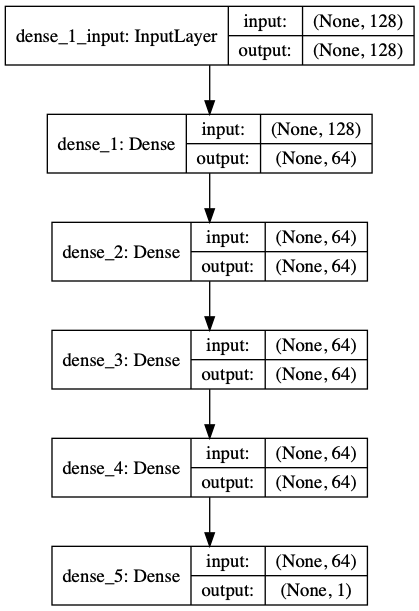
\includegraphics[width=2.5in]{../output/nn_model.png}
\end{minipage}
\begin{minipage}{0.5\linewidth}
\captionof{figure}{CNN model} \label{fig: cnn_model}
\centering
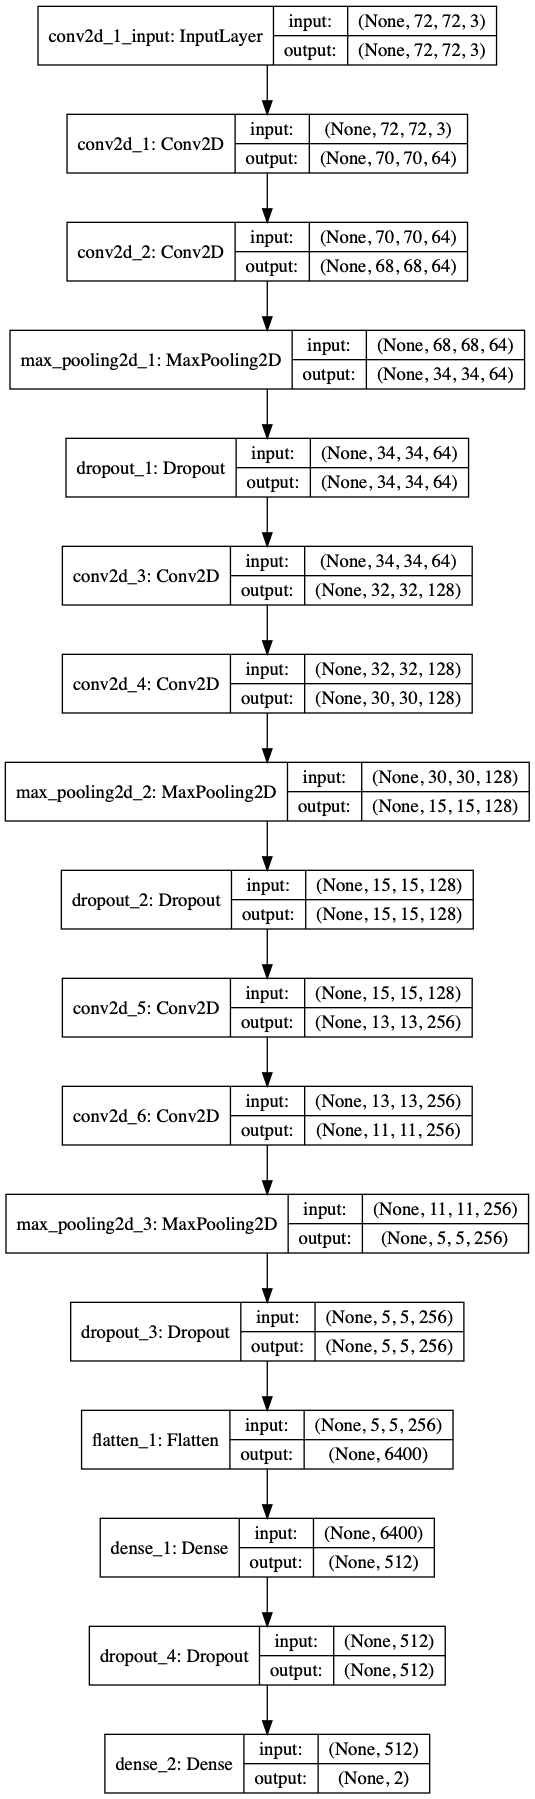
\includegraphics[width=2.5in]{../output/cnn_model.png}
\end{minipage}
\vspace*{10pt}

The relevant code for training any of the three models is in \texttt{train\_model()} in \texttt{face.py}. To train a gender classification model, run the command below.
\begin{minted}[bgcolor=bg]{sh}
python3 run.py train -m <model path after training> 
-c <classification model (SVM, NN_SIFT, or CNN)>
\end{minted}

The relevant code for face detection (including gender classification and face tracking) is in \texttt{face\_detection()} in \texttt{face.py}. Run the command below.
\begin{minted}[bgcolor=bg]{sh}
python3 run.py face_detection -i <input directory> -o <output directory>
-c <classification model (SVM, NN_SIFT, or CNN)> -m <trained model path> 
\end{minted}

\subsection*{Performance}
Table \ref{tab:gender_classification} shows the test accuracies of the three models. As expected, CNN performed poorly, achieving an accuracy that is equivalent to random guesses, due to the very small training data size of 468.

\begin{table}[h]
 \caption{Gender classification performance}
  \centering
  \begin{tabular}{lll}
    \toprule
    Model		& Description														& Accuracy on test set \\
    \midrule
    SVM							& 	Using SIFT descriptors of faces						& 100.00\% \\
    Neural network		& Using SIFT descriptors of faces							& 92.30\% \\
    CNN							&	Using cropped and resized faces						& 50.00\% \\
    \bottomrule
  \end{tabular}
  \label{tab:gender_classification}
\end{table}

\section{Make video}
The relevant code for combining all the frames to a video is in \texttt{make\_video()} in \texttt{utils.py}. To do logo detection, face detection, face tracking and gender classification and make a video, run the command below.
\begin{minted}[bgcolor=bg]{sh}
python3 run.py run_all -i <input directory> -o <output directory>
-d <logo path> -t <min threshold for NCC> -m <trained model path>
-c <classification model (SVM, NN_SIFT, or CNN)> -v <name of output video>
-f <frame per second>
\end{minted}

\section{References}
\href{https://www-nlpir.nist.gov/projects/tvpubs/tvpapers03/ramonlull.paper.pdf}{Video shot boundary detection based on color histogram}

\href{https://en.wikipedia.org/wiki/Shot_transition_detection}{Wikipedia - Shot transition detection}

\href{https://pdfs.semanticscholar.org/a662/2eed66acfddd9ba5ffe92b47c0af8ab335c3.pdf}{Shot detection using pixel wise difference with adaptive threshold and color histogram method in compressed and uncompressed video}

\newpage
\section{Code}
\foreach \file in  {shot, logo, face, utils, run} {
   %\begin{figure}[htpb]
        \lstinputlisting[language=Python, caption=\file.py]{../\file.py}
        %\caption{Source code for \textsf{\file.py}}
    % \label{fig:\file}
   %\end{figure}
}

\end{document}